\documentclass[12pt,a4paper]{article}
\usepackage[polish]{babel}
\usepackage[T1]{fontenc}
\usepackage[utf8x]{inputenc}
\usepackage{hyperref}
\usepackage{url}
\usepackage{graphicx}
\usepackage{float}

\addtolength{\hoffset}{-1.5cm}
\addtolength{\marginparwidth}{-1.5cm}
\addtolength{\textwidth}{3cm}
\addtolength{\voffset}{-1cm}
\addtolength{\textheight}{2.5cm}
\setlength{\topmargin}{0cm}
\setlength{\headheight}{0cm}

\begin{document}

\title{Sprawozdanie Grafika Komputerowa\\Opis interfejsu aplikacji: Foods}
\author{Krzysztof Czarnecki, 136224, WE, Informatyka}
\date{\today}

\maketitle

\tableofcontents

% zad 1
\section{Opis zamówienia}
\subsection{Przeznaczenie aplikacji}
Aplikacja ma służyć do zamawiania przez nas artykułów spożywczych z dowolnego sklepu. Osoba,
która będzie korzystała z aplikacji będzie mogła wybrać produkt np. chleb, następnie wybiera z jakiego
sklepu ten produkt ma być przywieziony. Oczywiście będzie miała wybór ze sklepów, które będą
dostępne aktualnie w aplikacji. Po złożeniu zamówienia, użytkownik otrzyma czas w jakim zamówienie
zostanie do niego dostarczone. Aplikacja działa na zasadzie zamówienie taksówki, tylko że zamawiamy
jedzenie.

\subsection{Opis Interfejsu}
Podczas otwierania aplikacji wyświetli się logo a następnie zostaniemy przeniesieni na stronę, w której
przy pierwszym rozpoczęciu będziemy musieli się zalogować i podłączyć kartę płatniczą. Na głównej
stronie trzeba będzie podać adres dostawy, chyba że pozwoliliśmy aplikacji na korzystanie z lokalizacji
telefonu. Następnie wybieramy jakie produkty chcemy zamówić, będzie wyświetlało się zdjęcie
produktu, cena, liczba oraz z jakiego sklepu zostanie przywieziony. Po dokonaniu wyboru otrzymamy
informacje w jakim czasie otrzymamy dostawę. Aplikacja w sidenavie będzie miała następujące pola:
Zamówienie, Płatności, historia zamówień, śledzenie aktualnej przesyłki, jeżeli dostawca będzie miał
opcje śledzenia , pomoc oraz informacje odnośnie aplikacji. W płatnościach możemy zmienić naszą
kartę płatniczą. W historii zamówienia będziemy mogli prześledzić nasze wszystkie zamówienia.

\subsection{Oprawa graficzna}
Szata graficzna w aplikacji będzie stała. Kolory, która będą przeważały to granatowy niebieski
połączony z białym. Czcionka będzie dosyć duża z racji tego, że aplikacja ma prostą budową i nie
posiada zbyt dużo funkcji.

\section{Pierwsza iteracja}
\subsection{Interfejs}
W pierwszej iteracji, na podstawie przedstawionych przez zamawiającego założeń, przygotowałem wstępny projekt interfejsu aplikacji. Poniżej przedstawiam pierwszą wersję aplikacji:

% logowanie v1 
\begin{figure}[H]
\centering
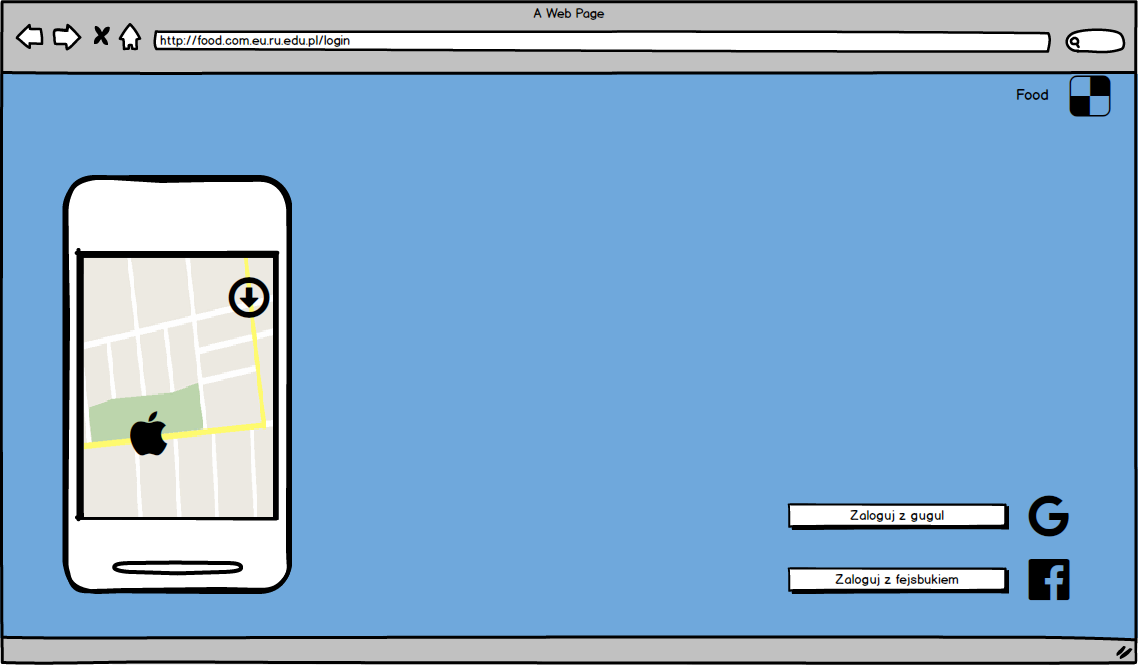
\includegraphics[width=15cm]{pictures/Logowanie_v0.png}
\caption{Ekran logowania}
\end{figure}

% lista produktów v1 
\begin{figure}[H]
\centering
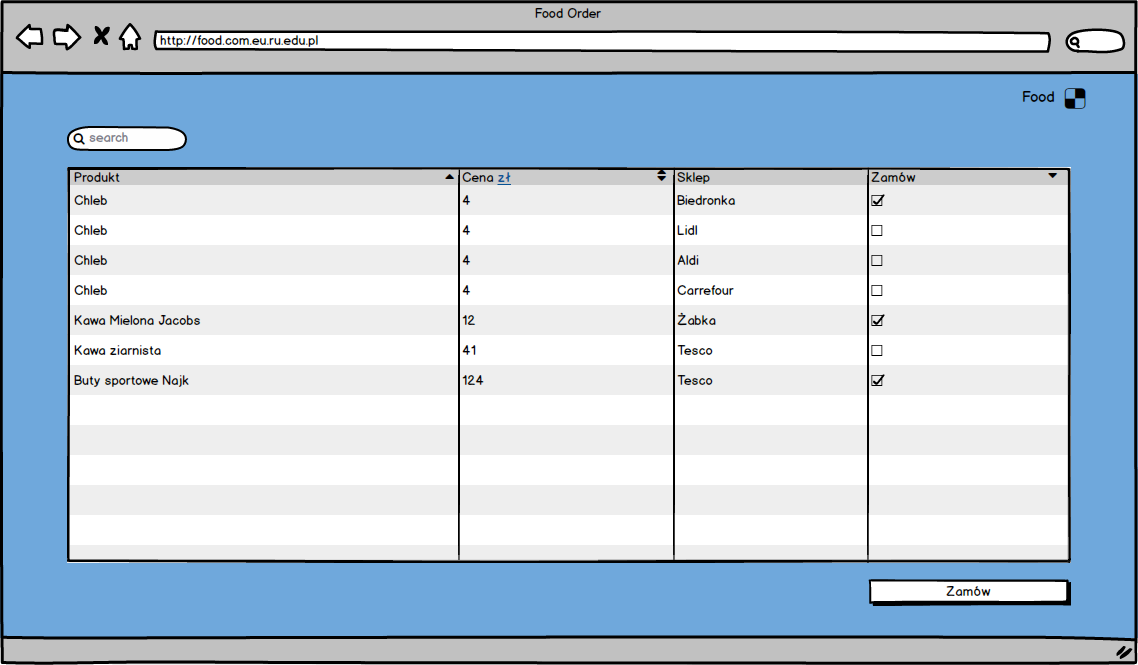
\includegraphics[width=15cm]{pictures/Lista_produktow_v1.png}
\caption{Ekran wyboru listy produktów}
\end{figure}

% lista produktów v1 
\begin{figure}[H]
\centering
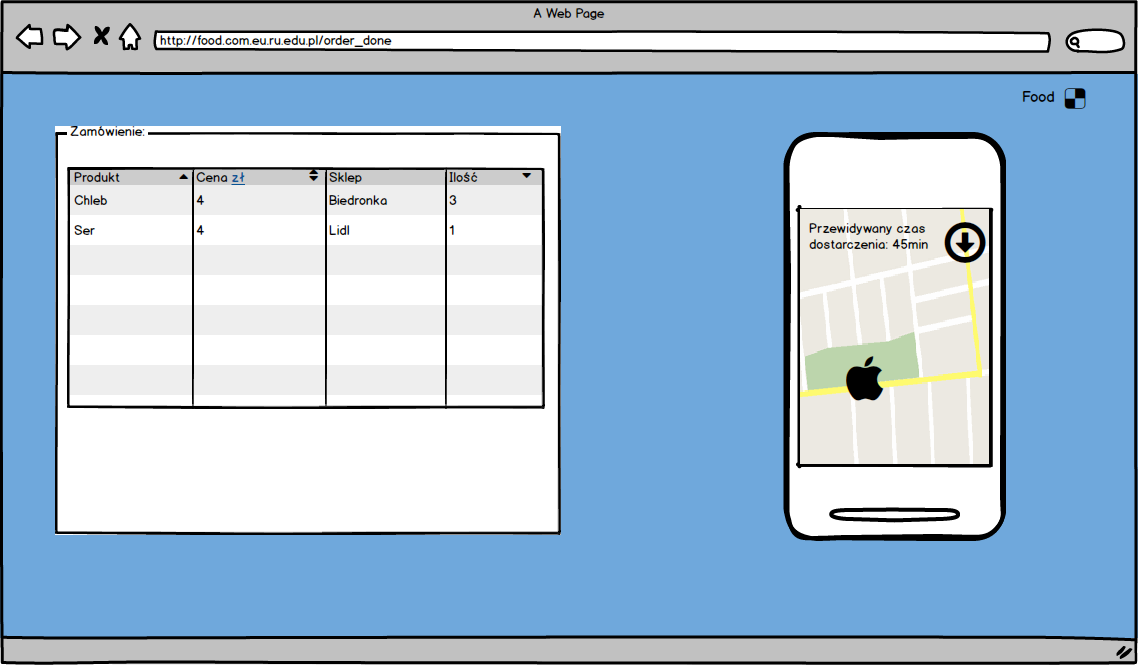
\includegraphics[width=15cm]{pictures/Zamowienie_zlozone_v1.png}
\caption{Ekran przedstawiający informację o złożonym zamówieniu i przewidywanym czasie dostawy}
\end{figure}

\subsection{Uwagi zamawiającego}
Po przedstawieniu zamawiającemu pierwszej wersji interfejsu, stwierdził on, iż aplikacja ma właściwą szatę kolorystyczną. Chciałby jednak, aby lista produktów była wykonana w bardziej przejrzysty i łatwiejszy w obsłudze sposób. W pierwszej iteracji zostały przedstawione zamawiającemu najważniejsze okna w systemie.


\section{Druga iteracja}
\subsection{Interfejs}
W drugiej iteracji poprawiony został wygląd strony przedstawiający listę produktów. Aktualnie najważniejszym aspektem charakteryzującym pojedynczą kolumnę w tabeli jest produkt, a nie jak w poprzedniej wersji złączenie produktu ze sklepem. W efekcie uzyskaliśmy efekt widoczny na poniższej grafice:

\begin{figure}[H]
\centering
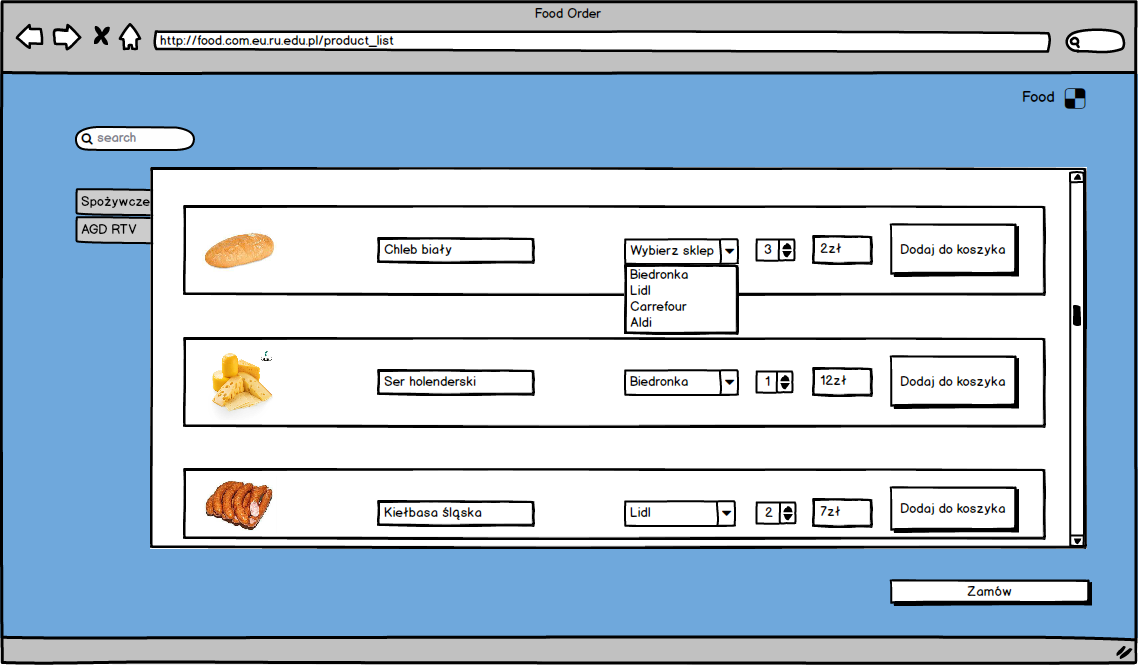
\includegraphics[width=15cm]{pictures/Lista_produktow_v2.png}
\caption{Druga iteracja wyboru produktu.}
\end{figure}

\begin{figure}[H]
\centering
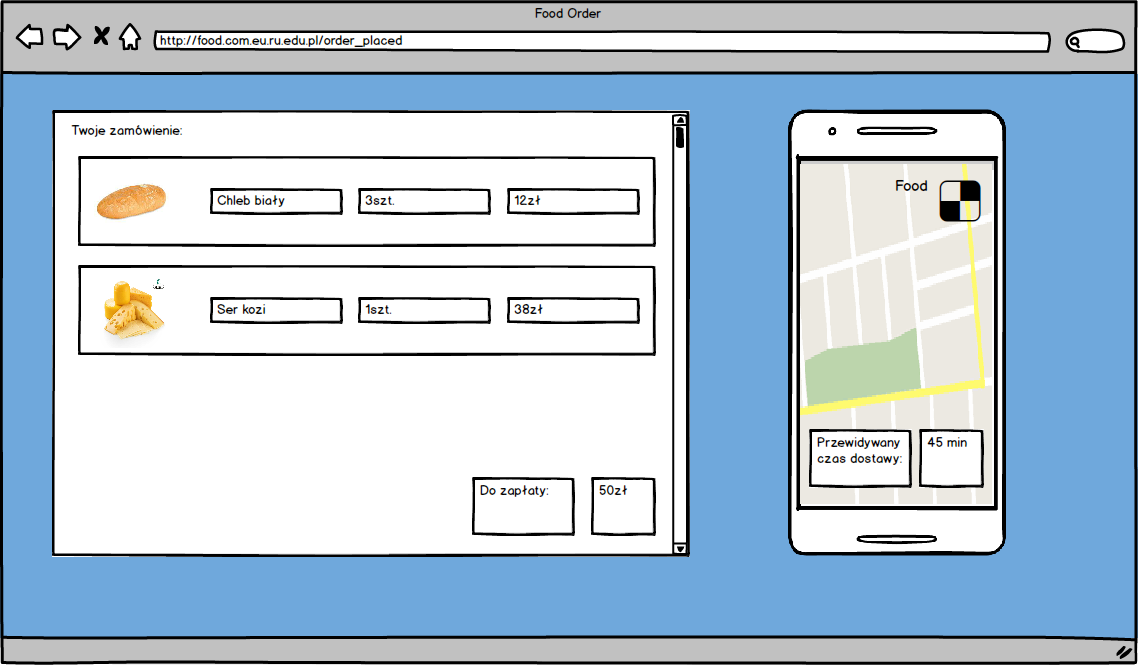
\includegraphics[width=15cm]{pictures/Zamowienie_zlozone_v2.png}
\caption{Druga iteracja ekranu złożonego zamówienia.}
\end{figure}

\subsection{Uwagi zamawiającego}
Klient zaakceptował widok w drugiej iteracji. Pragnął jednak, aby na każdym ekranie widoczny był taki sam \textit{header} z rozsuwanym menu, tzw. \textit{menu hamburger}.

\section{Trzecia iteracja}
\subsection{Interfejs}
Trzecia iteracja dogadywania szczegółów z klientem zawiera dodatkowy \textit{header} oraz przedstawione rozsunięte \textit{menu hamburger}.

\begin{figure}[H]
\centering
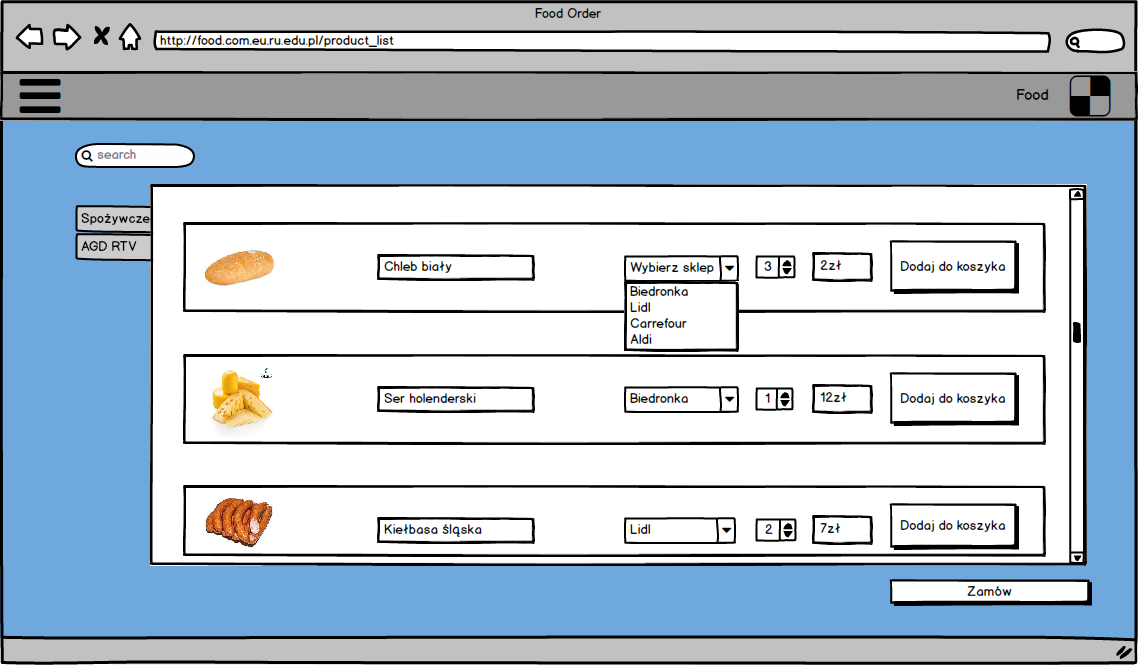
\includegraphics[width=15cm]{pictures/Lista_produktow_v3.png}
\caption{Trzecia iteracja wyboru listy produktów.}
\end{figure}

\begin{figure}[H]
\centering
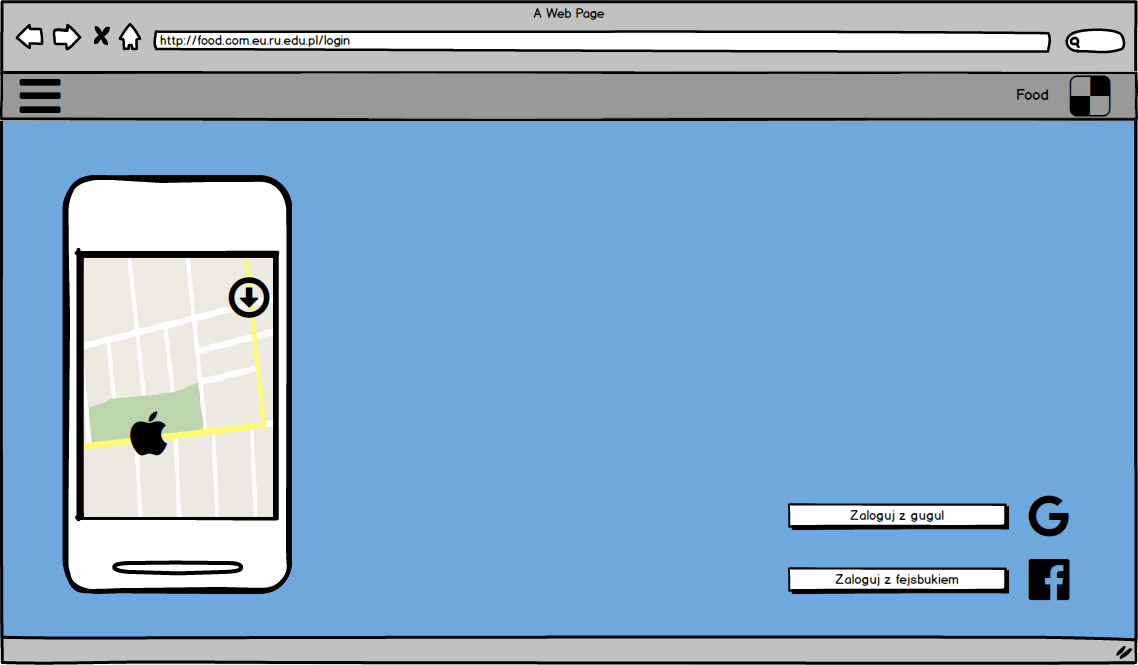
\includegraphics[width=15cm]{pictures/Logowanie_v1.png}
\caption{Ekran logowanie w trzeciej iteracji.}
\end{figure}

\begin{figure}[H]
\centering
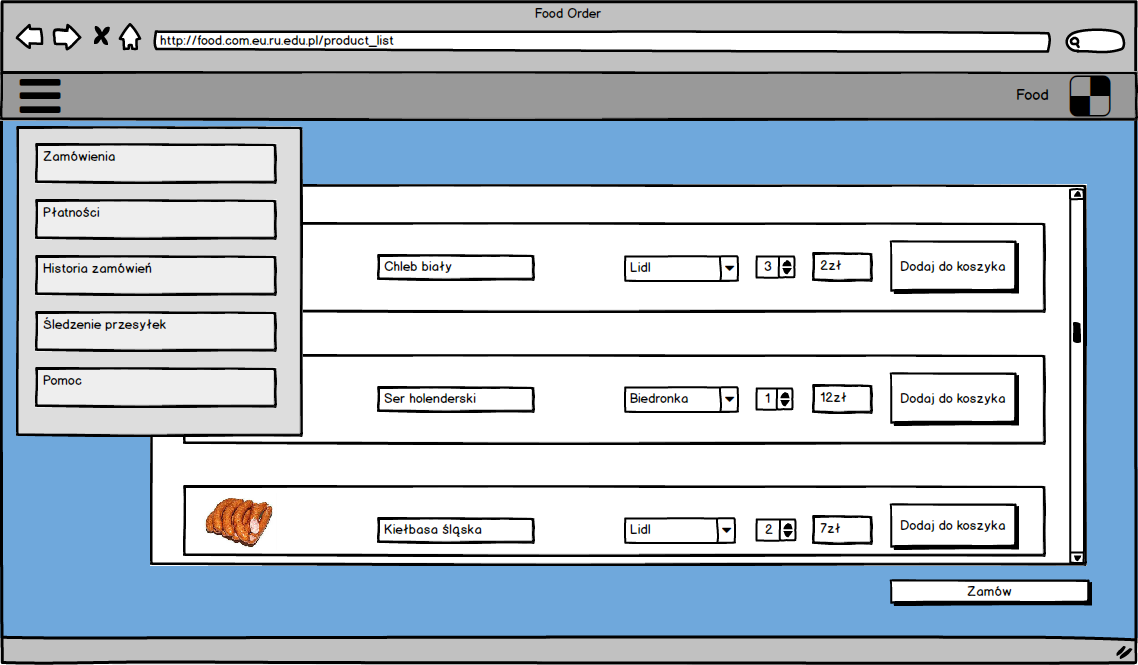
\includegraphics[width=15cm]{pictures/Navbar_v1.png}
\caption{Rozsunięte \textit{menu hamburger}.}
\end{figure}

\begin{figure}[H]
\centering
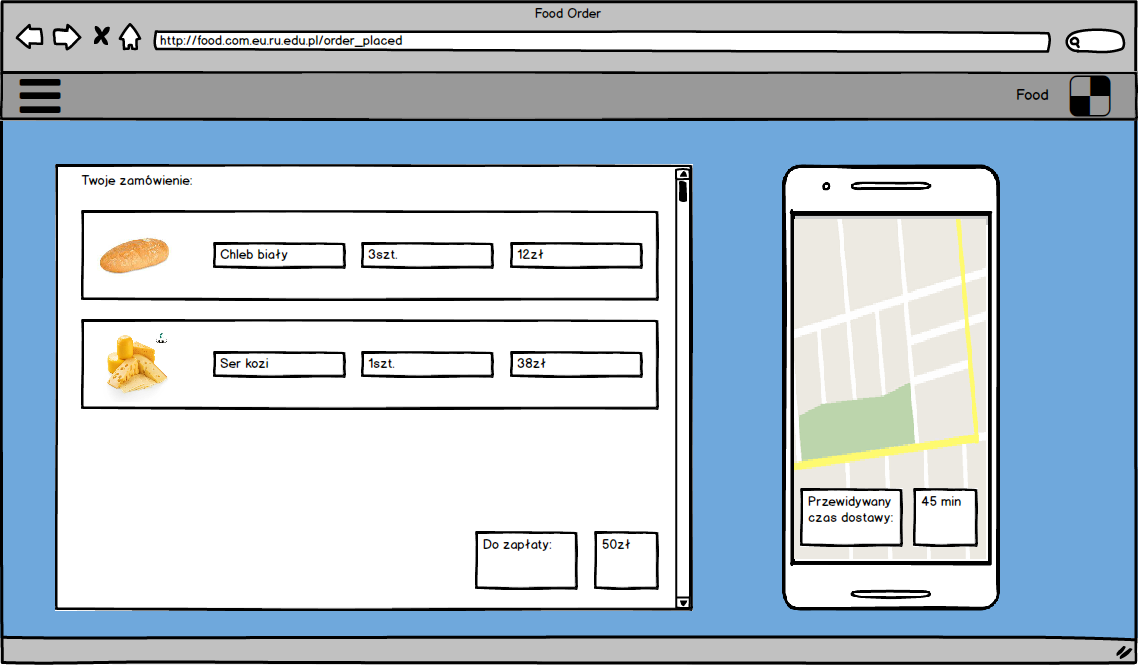
\includegraphics[width=15cm]{pictures/Zamowienie_zlozone_v3.png}
\caption{Ekran złożonego zamówienia.}
\end{figure}

\subsection{Uwagi zamawiającego}
Zamawiający prosił jeszcze o zmianę obrazu telefonu na ekranie logowania na bardziej współczesny, identyczny do tego, który widnieje na ekranie złożonego zamówienia oraz o przedstawienie ekranu śledzenia przesyłek.


\section{Efekt końcowy}
\subsection{Interfejs}

\begin{figure}[H]
\centering
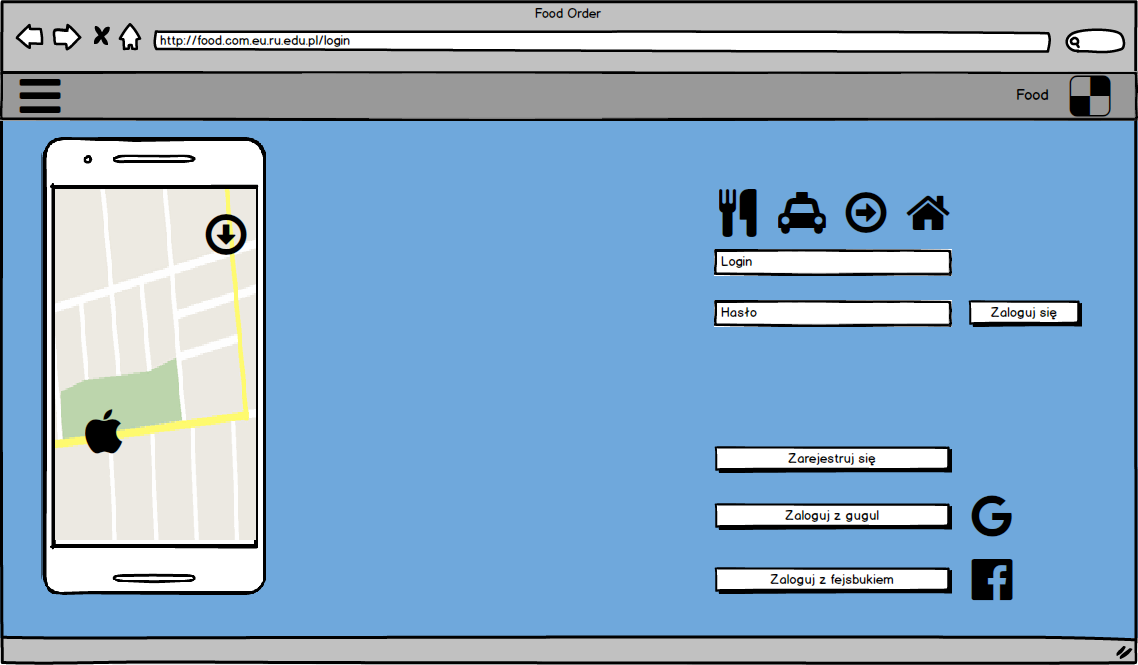
\includegraphics[width=15cm]{pictures/Logowanie_v2.png}
\caption{Efekt końcowy - ekran logowania.}
\end{figure}

\begin{figure}[H]
\centering
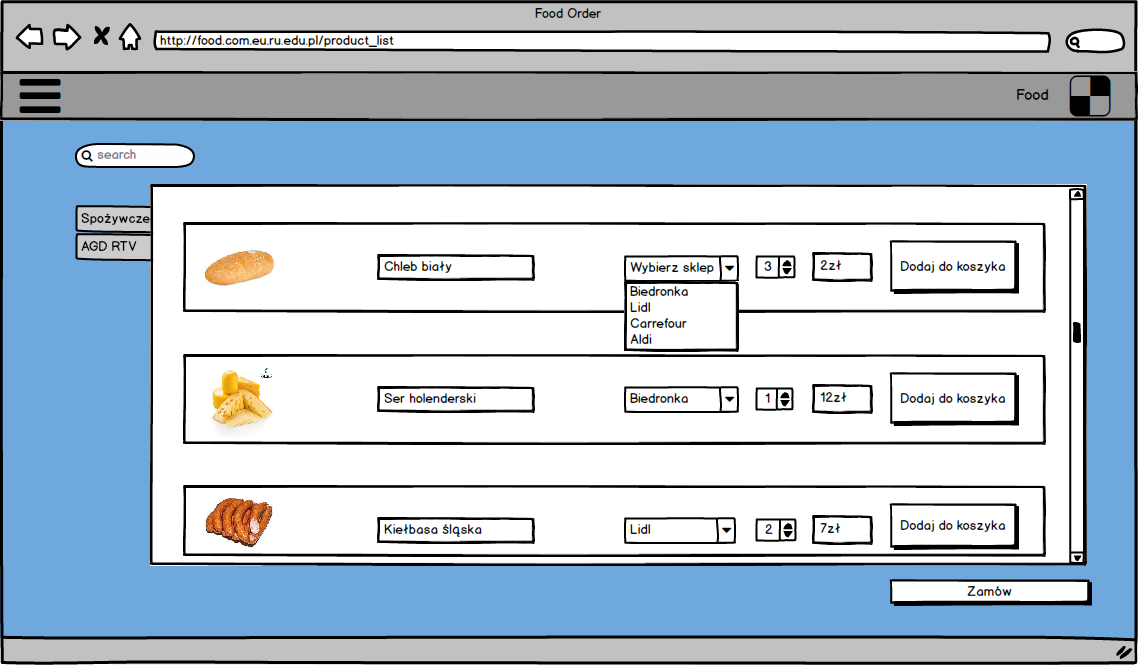
\includegraphics[width=15cm]{pictures/Lista_produktow_v3.png}
\caption{Efekt końcowy - lista produktów.}
\end{figure}

\begin{figure}[H]
\centering
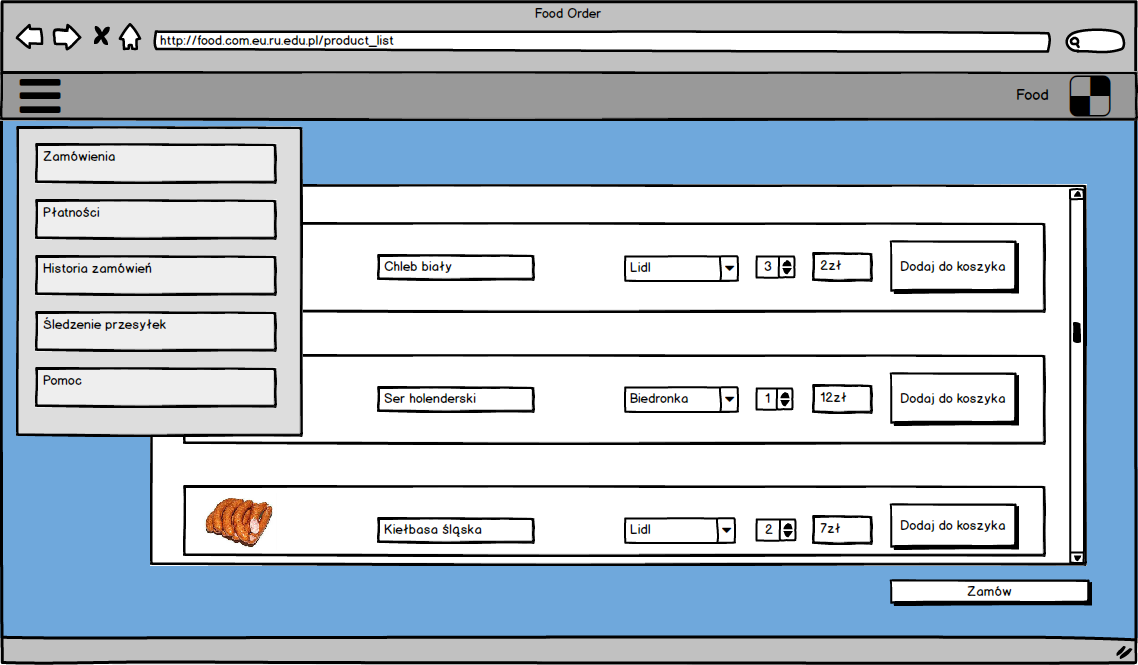
\includegraphics[width=15cm]{pictures/Navbar_v1.png}
\caption{Efekt końcowy - rozsunięte \textit{menu hamburger}.}
\end{figure}

\begin{figure}[H]
\centering
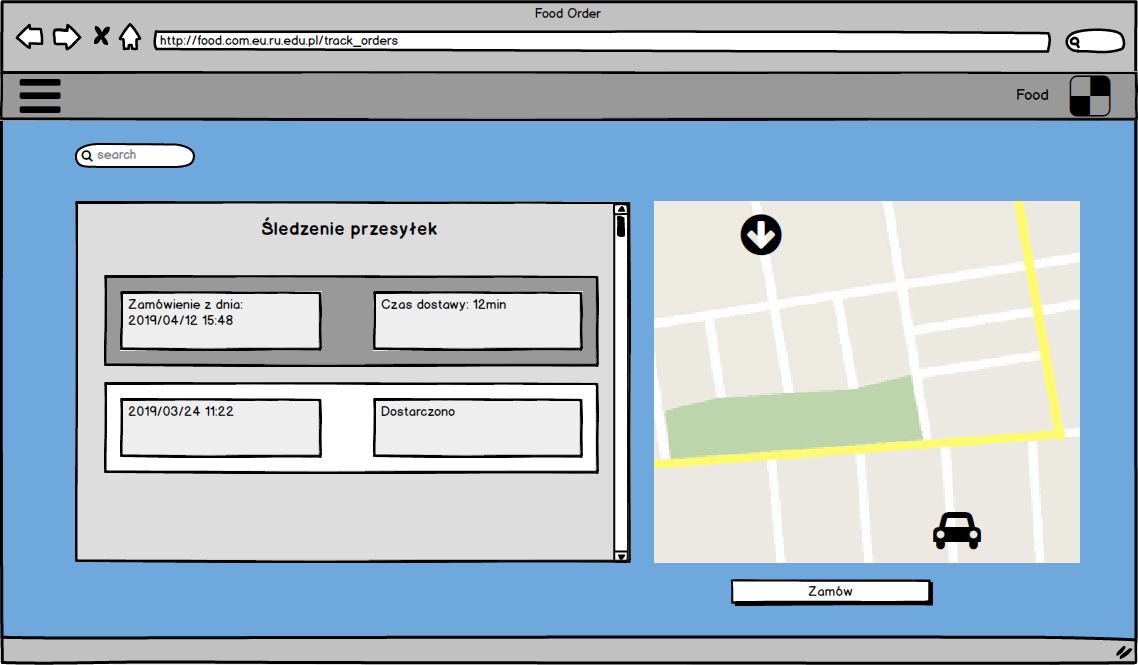
\includegraphics[width=15cm]{pictures/sledzenie_przesylek_v1.png}
\caption{Efekt końcowy - ekran śledzenia przesyłek.}
\end{figure}

\begin{figure}[H]
\centering
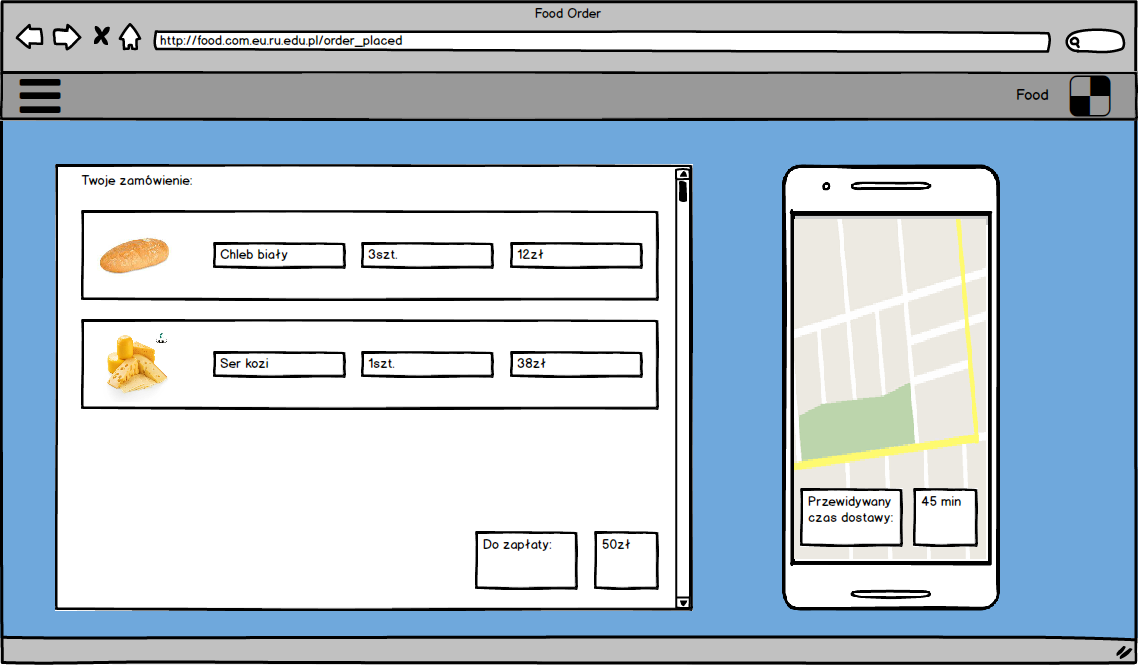
\includegraphics[width=15cm]{pictures/Zamowienie_zlozone_v3.png}
\caption{Efekt końcowy - ekran złożonego zamówienia.}
\end{figure}

\subsection{Ocena zamawiającego}
Poniżej cytat oceny interfejsu przez zamawiającego:
\begin{quote}
Aplikacja spełnia moje oczekiwania. Wyglada bardzo estetycznie i prosto tak jak zaplanowałem. W skali 5'cio punktowej skali oceniam ją na 4,5. 
\end{quote}

\end{document}

% PUNKTORY
% \begin{itemize}
% \item Public Documents
% \item All Documents
% \item Create Document
% \end{itemize}

% obrazek
% \begin{figure}[H]
% \centering
% \includegraphics[width=15cm]{pictures/deszyf_mycbc.png}
% \caption{Wykres zależności czasu deszyfrowania [ms] od wielkości pliku [MB] z uwzględnieniem własnej implementacji szyfru CBC}
% \label{pictures/szyfrowanie.png}
% \end{figure}